% Source: AESP_466_ClassWork/Supplements/Notes/latex/5.3.4/5.3.4.tex

\documentclass[border=4pt]{standalone}
\usepackage{amsmath,amssymb,amsthm}
\usepackage{graphicx}
\usepackage{tikz}
\usepackage{xcolor}
\usetikzlibrary{arrows.meta,calc,positioning,decorations.markings,patterns,shapes.geometric,angles,quotes}

\definecolor{Garnet}{HTML}{73000A}
\definecolor{USC_Rose}{HTML}{CC2E40}
\definecolor{USC_Blue}{HTML}{466A9F}
\definecolor{USC_Slate}{HTML}{1F414D}
\definecolor{USC_Olive}{HTML}{65780B}
\definecolor{USC_Lime}{HTML}{CED318}
\definecolor{USC_Gold}{HTML}{A49137}
\definecolor{USC_Black90}{HTML}{565556}
\definecolor{USC_Black10}{HTML}{ECECEC}

\newcommand{\vect}[1]{\mathbf{#1}}
\newcommand{\mat}[1]{\mathbf{#1}}
\newcommand{\uvec}[1]{\hat{\mathbf{#1}}}
\newcommand{\transpose}{^{\mkern-1.5mu\mathsf{T}}}
\newcommand{\inv}{^{-1}}
\newcommand{\deriv}[2]{\frac{d #1}{d #2}}
\newcommand{\pderiv}[2]{\frac{\partial #1}{\partial #2}}

\begin{document}
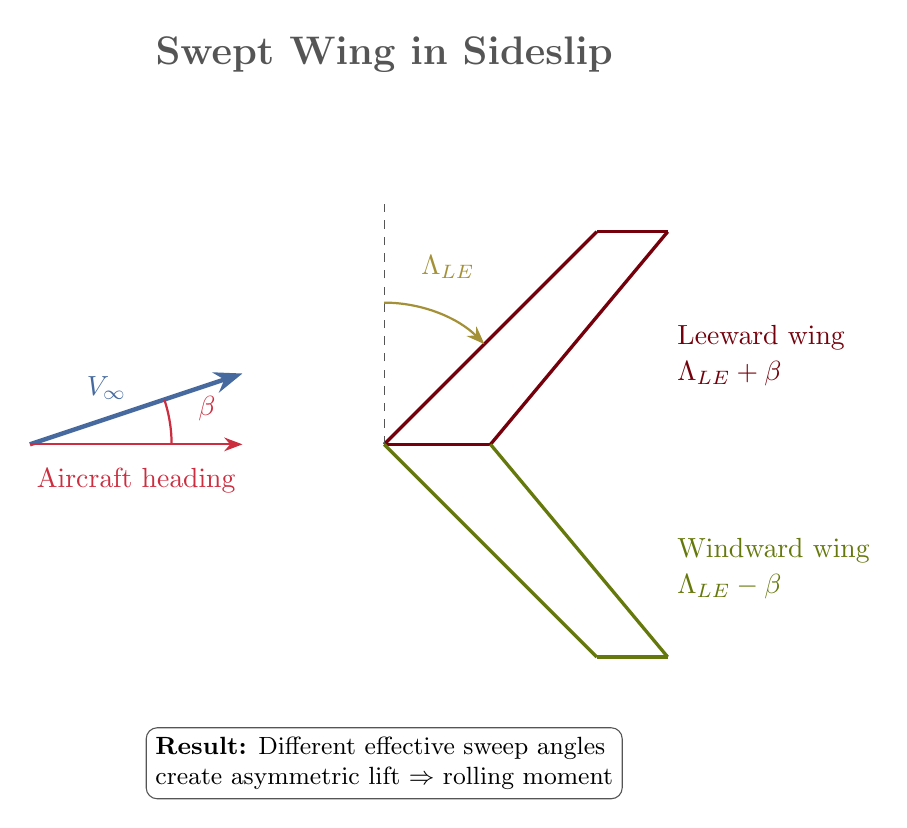
\begin{tikzpicture}[>=Stealth, scale=0.9]
    % Title
    \node[font=\Large\bfseries, USC_Black90] at (0,5.5) {Swept Wing in Sideslip};

    % Freestream velocity (with sideslip)
    \draw[->, ultra thick, USC_Blue] (-5,0) -- (-2,1);
    \node[USC_Blue, above left] at (-3.5,0.5) {$V_\infty$};

    % Sideslip angle arc
    \draw[->, thick, USC_Rose] (-5,0) -- (-2,0);
    \node[USC_Rose, below] at (-3.5,-0.2) {Aircraft heading};
    \draw[thick, USC_Rose] (-3,0) arc (0:18.4:2);
    \node[USC_Rose] at (-2.5,0.5) {$\beta$};

    % Wing planform (swept)
    % Right wing (leeward in positive sideslip)
    \draw[very thick, Garnet] (0,0) -- (3,3);
    \draw[very thick, Garnet] (1.5,0) -- (4,3);
    \draw[very thick, Garnet] (0,0) -- (1.5,0);
    \draw[very thick, Garnet] (3,3) -- (4,3);
    \node[Garnet, right] at (4,1.5) {Leeward wing};
    \node[Garnet, right] at (4,1) {$\Lambda_{LE} + \beta$};

    % Left wing (windward in positive sideslip)
    \draw[very thick, USC_Olive] (0,0) -- (3,-3);
    \draw[very thick, USC_Olive] (1.5,0) -- (4,-3);
    \draw[very thick, USC_Olive] (3,-3) -- (4,-3);
    \node[USC_Olive, right] at (4,-1.5) {Windward wing};
    \node[USC_Olive, right] at (4,-2) {$\Lambda_{LE} - \beta$};

    % Sweep angle annotation
    \draw[dashed, USC_Black90] (0,0) -- (0,3.5);
    \draw[->, thick, USC_Gold] (0,2) arc (90:45:2);
    \node[USC_Gold] at (0.9,2.5) {$\Lambda_{LE}$};

    % Annotation box
    \node[draw=USC_Black90, fill=white, rounded corners, align=left, font=\small] at (0,-4.5) {
        \textbf{Result:} Different effective sweep angles\\
        create asymmetric lift $\Rightarrow$ rolling moment
    };

\end{tikzpicture}
\end{document}
